%%%%%%%%%%%%%%%%%%%%%%%%%%%%%% -*- Mode: Latex -*- %%%%%%%%%%%%%%%%%%%%%%%%%%%%
%% 10-05.tex --      IEEE Smart Grid Comm paper
%% Author          : Philip Johnson
%% Created On      : Mon Sep 23 11:52:28 2002
%% Last Modified By: Philip Johnson
%% Last Modified On: Fri Apr 16 15:19:50 2010
%%%%%%%%%%%%%%%%%%%%%%%%%%%%%%%%%%%%%%%%%%%%%%%%%%%%%%%%%%%%%%%%%%%%%%%%%%%%%%%
%%   Copyright (C) 2009 Philip Johnson
%%%%%%%%%%%%%%%%%%%%%%%%%%%%%%%%%%%%%%%%%%%%%%%%%%%%%%%%%%%%%%%%%%%%%%%%%%%%%%%
%% 

%% Home page: http://www.ieee-smartgridcomm.org/submission.html

%% Must submit to one of the 12 symposia:
%% http://www.ieee-smartgridcomm.org/symposia.html

%% It appears that this is the most relevant symposia:
%% http://www.ieee-smartgridcomm.org/hibfn.html

%% For ``peer review mode'', do:
%%   \documentclass[conference,compsoc,peerreview]{IEEEtran}
%% and
%%   \IEEEpeerreviewmaketitle  (after the abstract).

%\documentclass[conference,compsoc,peerreview]{IEEEtran}
\documentclass[conference]{IEEEtran}
\usepackage[final]{graphicx}
\usepackage{cite}
\usepackage{url}
% uncomment the % away on next line to produce the final camera-ready version
% and uncomment the \thispagestyle{empty} following \maketitle
%\pagestyle{empty}

\begin{document}

\title{WattDepot: An open source software ecosystem for enterprise-scale
  energy data collection, storage, analysis, and visualization}

\author{Robert S. Brewer\\
        Philip M. Johnson\\
\em     Collaborative Software Development Laboratory\\
        Department of Information and Computer Sciences\\
        University of Hawai`i at M\=anoa\\
        Honolulu, HI 96822\\
        rbrewer@lava.net, johnson@hawaii.edu\\
}


\maketitle
%\IEEEpeerreviewmaketitle
%\thispagestyle{empty}

\begin{abstract}  % 200 words
  WattDepot is an open source, Internet-based, service-oriented framework 
  for collection, storage, analysis, and visualization of energy data.
  WattDepot differs from other energy management solutions in one or more
  of the following ways: it is not tied to any specific metering
  technology; it provides high-level support for meter aggregation and data
  interpolation; it supports carbon intensity analysis; it is
  architecturally decoupled from the underlying storage technology; it
  supports both hosted and local energy services; it can provide near-real
  time data collection and feedback; and the software is open source and
  freely available.  In this paper, we introduce the framework, provide
  examples of its use, and discuss its application to research and
  understanding of the Smart Grid.
\end{abstract}


\section{Introduction}
\label{sec:intro}

Recent interest in the Smart Grid has produced a wide variety of proposed
``open'' standards and technologies for energy data collection, storage,
and analysis.  Some prominent approaches include cloud-based services like
Google PowerMeter \cite{GooglePowerMeter} and Microsoft Hohm
\cite{MicrosoftHohm}, ``interoperable'' protocols and networking approaches
like Smart Energy 2.0 \cite{SmartEnergy2.0} and GridRouter Ecosystem
\cite{GridRouterEcosystem}, smart grid standards like IEEE SCC21
\cite{IEEESCC21} and Oasis Blue \cite{OasisBlue}, extensible energy
management devices like Control4's EMS 100 \cite{EMS100}, and home energy 
meters like the TED 5000 \cite{TED}.  There are also
``open source'' hardware platforms, such as OSHAN \cite{OSHAN}, and open
source software solutions for phasor data such as OpenPDC \cite{OpenPDC}.

For our research on behavioral change among energy consumers in a building
or home environment, we need a way to: (a) collect energy data from a
variety of meters with the possibility of near-real time (5-10 second)
feedback, (b) store the results in an Internet-accessible repository; (c)
perform basic analyses on the raw data including aggregation and
interpolation, and (d) visualize the raw and processed data in a variety of
ways, including tables, gauges, trend lines, geographic maps, heat maps, and so forth.

Unfortunately, we find that none of the current ``open'' technologies
satisfy these seemingly simple requirements. Either the technology is
designed for a specific brand of meter (such as the EMS 100 or TED 5000), or it does not
support near-real time feedback (such as Google PowerMeter and Microsoft
Hohm), or it focuses on utility issues (OpenPDC), or it focusses on
wire-level or hardware concerns (OSHAN, GridRouter Ecosystem).


\begin{figure*}[!th]
  \center
  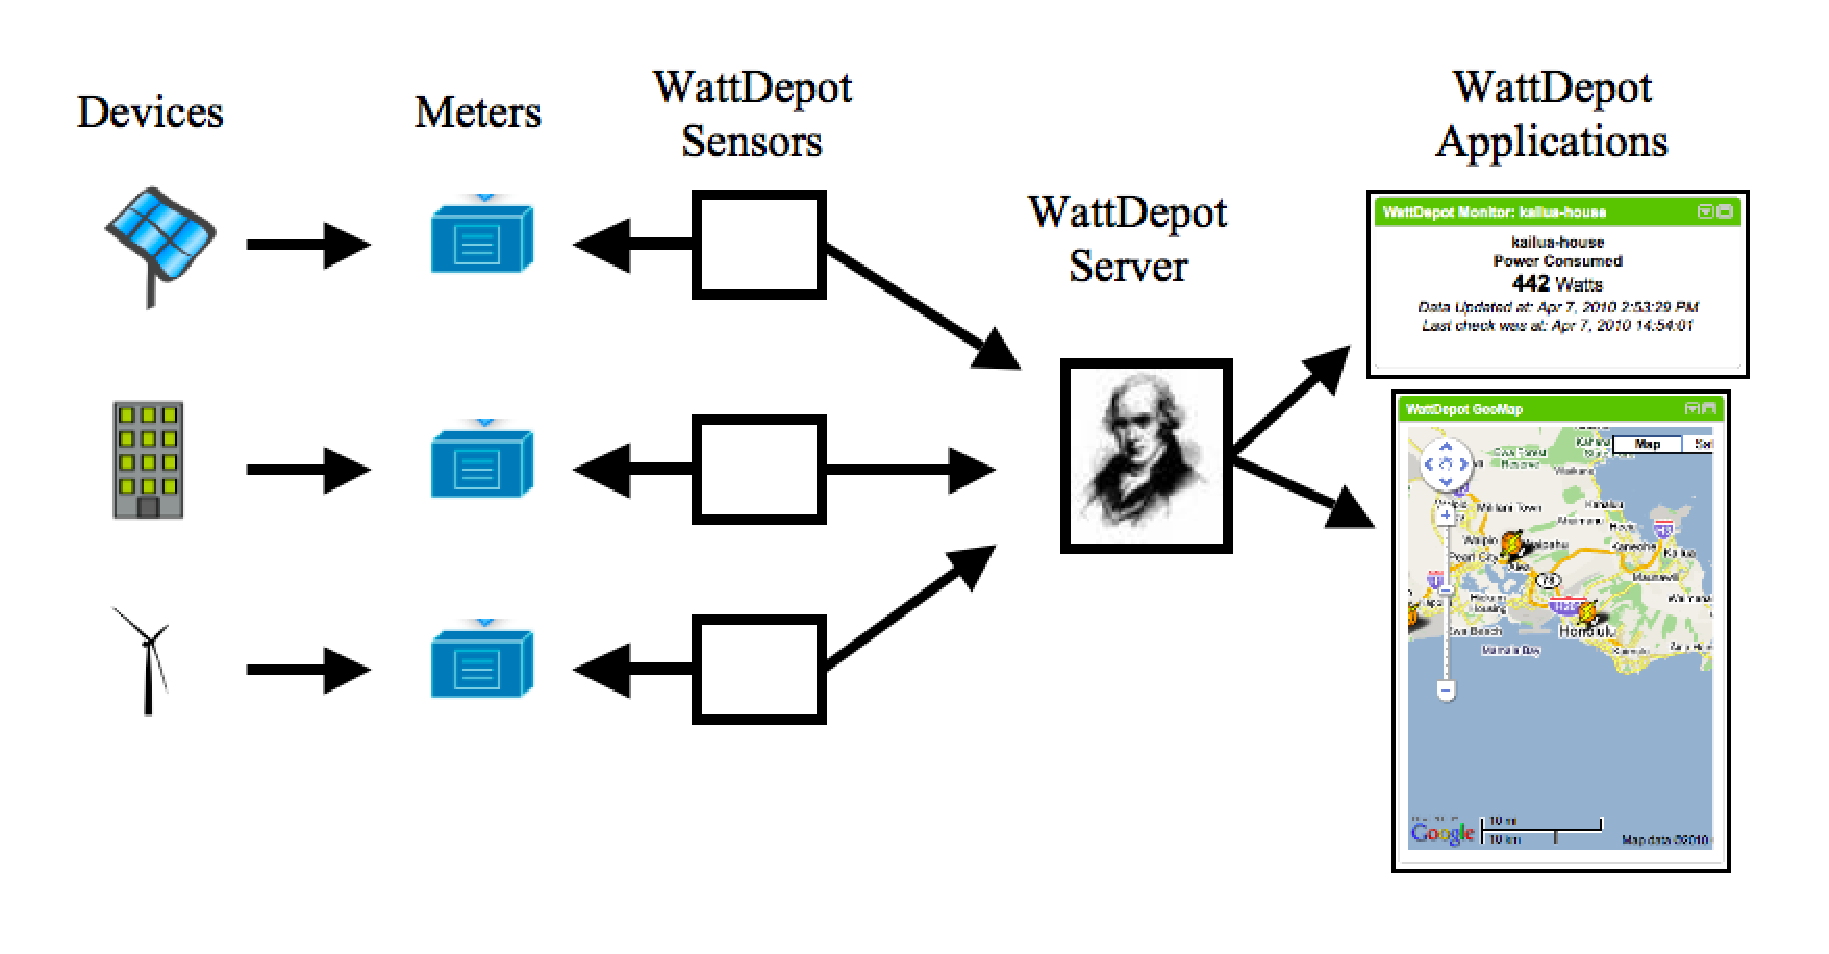
\includegraphics[width=0.8\textwidth]{architecture.eps}
  \caption{\em \small Architecture of WattDepot: sensors obtain data from
    meters on consumption or generation, transmit their findings to a
    server, which is queried by clients to present visualizations or analyses.}
  \label{fig:architecture}
\end{figure*} 

Rather than implement a special purpose solution for our research, we
decided to leverage our prior experience in open source software
engineering measurement systems to design and implement an open source,
extensible, service-oriented framework for energy data collection, storage,
analysis, and visualization. Our framework, called WattDepot, consists of
three kinds of services:

\begin{itemize}
\item WattDepot {\em sensors}, each customized for a particular brand of
energy meter.  A sensor requests data from a meter according to the meter's
protocol, then sends it to a WattDepot repository for storage.

\item WattDepot {\em repositories}, which implement a REST \cite{REST} API
for accepting energy data sent from sensors and providing this sensor data
(or analyses based upon the data) to WattDepot clients.

\item WattDepot {\em clients}, which request data from WattDepot
repositories and either display the data or analyses directly to users or
provide the data to higher level energy services.
\end{itemize}

\figurename \ref{fig:architecture} illustrates the architecture of the system.


For example, consider a University that wants to implement a dorm energy
competition in which energy meters will be installed on each floor of the
dorm and residents of each floor will compete against each other to see who
can reduce their energy the most.  Prior to WattDepot, one could either buy a
proprietary, ``black box'' solution such as the Building Dashboard from
Lucid Design Group and be restricted to the set of meters and analyses they
support, or else start from scratch and build all of the energy data
collection, analysis, and visualization services.  WattDepot provides an
alternative approach, in which collection, storage, and analysis
capabilities are freely available and amenable to integration within a web
application developed by the user.  For those with some software
development capability, this can be a lower cost solution and/or support
customization beyond the ability of current proprietary solutions.

WattDepot services are designed at the ``enterprise'' scale as opposed to
the ``home'' or ``utility'' scales.  By home scale, we mean systems like
the TED 5000, which are designed to collect and analyze data about a single
residence, typically through a simple ``dashboard'' interface that runs on
the user's local area network.  WattDepot is designed to
collect, store, and analyze data from a wider range of locations using the
Internet as the transmission mechanism, and our performance analysis tests
indicate that it can easily process several thousand sensor data storage
requests per minute given adequate network bandwidth.  On the other hand,
by utility scale, we mean systems that can collect and store grid-level
data comprising tens or hundreds of thousands of residences, with
revenue-grade measurement, hardened storage, and security mechanisms.
WattDepot is not intended for these more rigorous utility-level
requirements.  Our goal for WattDepot is to provide a mechanism to
accelerate innovative research and development in energy analysis and
visualization by providing an extensible architecture and well documented,
open source software platform.

The next section of this paper introduces the basic components of
WattDepot. Following this we describe some of our initial experiences with
the framework and conclude with our future directions. 

\section{WattDepot Services}

\subsection{Sensors}

Electricity can be generated and/or consumed by a wide variety of devices
and monitored by a wide variety of metering technologies.  Many energy
management software systems are tied to a particular energy device and/or
meter; indeed, they are often marketed as an accessory to the hardware.  For
example, a solar panel company might provide software for storing data
about the power generated by the panel and simple visualizations of the
power generated over time.

The design of WattDepot attempts to make the software as independent from
the energy hardware devices as possible.  In WattDepot, it is the device
that is the accessory to the software.  To achieve this independence, the
WattDepot architecture includes ``sensors'', or small software processes
that query any given energy device according to its native protocol,
collect standard information, and then send it to a WattDepot server using
the Internet and the RESTful WattDepot API over HTTP.  This design means
that new energy devices can be integrated easily into the WattDepot
software ecosystem just by writing the sensor interface.  The use of a
RESTful HTTP protocol for communication with the WattDepot server means
that the sensor can be implemented in any programming language.

We have implemented WattDepot sensors for the TED 5000 home energy device, 
the Veris power meter collected through the Building Manager Online system,
and for the Acuvim energy meter. This latter sensor is particularly
interesting because it is communicates with the meter through the standard
ModBus/TCP protocol. The sensor is designed in a modular way so that it is
easy to customize to support other meters that communicate using ModBus/TCP.

Sensors transmit data to a WattDepot server using a standardized, published
protocol, as discussed next.

\subsection{Servers}

A WattDepot server accepts raw energy data from devices (via sensors) and
makes this data (or analyses based upon it) available to clients.  The
WattDepot server implements a variety of design decisions intended to
improve its generality, reusability, and extensibility, including: (1) a
RESTful API, (2) a pluggable back-end database, (3) aggregation via
``virtual'' sources, (4) data interpolation, and (5) multiple
representations.

{\em RESTful API.} WattDepot conforms to modern web service design best
practices by providing a RESTful API.  REST (REpresentational State
Transfer) \cite{REST} is a specification paradigm, which, when applied to
web services, generally results in more easily usable and extensible
communication than alternatives such as SOAP. The details of RESTful design
are beyond the scope of this paper, but some of the implications are that
URLs can serve as unique identifiers for energy data and that HTTP commands
such as PUT, POST, GET, and DELETE are used to add, amend, retrieve, and
delete energy data. The WattDepot API \cite{WattDepotAPI} provides more
details and a full specification of the supported operations.

{\em Pluggable back-end database.} The WattDepot server implements an
abstraction layer that enables the server to be built with a variety of
different persistence mechanisms.  By default, WattDepot uses the Apache
Derby relational database, which is a high performance, embedded database
written in Java.  However, WattDepot can be ported to other relational or
non-relational database systems by implementing an interface and setting some 
run-time configuration parameters. 

{\em Aggregation via virtual sources.} The data from a single physical
meter is generally represented in WattDepot as a ``Source''.  Each
WattDepot Source can indicate the power generated or consumed by that
device at any moment in time, the energy generated or consumed by that
device over a period of time, the carbon intensity associated with that
device, and other features.  In addition to this one-to-one correspondence,
WattDepot also supports the definition of ``virtual'' Sources, which are
Sources defined as the aggregation of other Sources.  For example, a floor
on a building might have two meters collecting data about energy
consumption for the two sections of the floor.  WattDepot allows users to
define a virtual Source representing the aggregation of the data stream
from the two meters.  This virtual Source thus represents the total energy
consumption for the floor. Virtual Sources can be arranged in a hierarchy,
such that the virtual Sources for each floor in the building can themselves
be contained in a virtual Source representing the entire building's energy
consumption.

{\em Data interpolation.} One common initial roadblock to analyzing energy
data collected from multiple sources is the ``timestamp problem''. For
example, assume that energy consumption on a building floor is collected by
two meters, and that energy data is collected from those meters becomes
available approximately every 15 minutes, but the timestamps associated
with the data for a given time period differ by a minute or two.
Determining the aggregate energy consumption is no longer a simple matter
of importing the two data sets into a spreadsheet and using a summation
macro, because the timestamps from the two meters do not ``match up''.
WattDepot addresses this problem by providing automatic interpolation. For
example, assume a meter sent energy data at roughly 30 minute intervals:
11:23 AM, 11:56 AM, 12:25 PM, and 1:01 PM.  You can request the energy consumed
by this Source between 12:00 PM and 1:00 PM, for example, and WattDepot will
automatically interpolate the raw data values to provide an estimate for
the interval of interest.  Automatic linear interpolation enables virtual Sources
to return reasonable values even when its constituent Sources send data at
different times and with different frequencies.  \figurename \ref{fig:visualizer}
illustrates both virtual sources and data interpolation. 

{\em Multiple representations.} One benefit of a RESTful architecture is
the separation of a ``resource'' from its ``representation''.  In
WattDepot, this means that data and analyses for a given Source can be
provided in different ways, depending upon the needs of the client.  So
far, WattDepot can provide data to clients using XML, JSON (the format
supported by Google Visualizations), and CSV (comma-separated values),
which is useful for importing WattDepot data into other tools for
additional analysis.

\subsection{Clients}

While sensors collect energy data, and the server stores, aggregates, and
interpolates it, WattDepot clients extract the data for presentation to the
user or input into tools for additional analysis.  The WattDepot RESTful
API is designed to enable a wide variety of clients to easily interact with
WattDepot energy data.  

\begin{figure}[thb]
  \center
  \includegraphics[width=0.48\textwidth]{monitor.eps}
  \caption{\em \small The WattDepot monitor client displaying the latest sensor
  data for a home.}
  \label{fig:monitor}
\end{figure}

\begin{figure*}[!th]
  \center
  \includegraphics[width=0.6\textwidth]{visualizer.eps}
  \caption{\em \small The WattDepot Visualizer client displaying a virtual Source
    (in blue) for a building floor and its two constituent physical Sources (in red and orange) corresponding to energy meters. All data values are interpolated.}
  \label{fig:visualizer}
\end{figure*} 

\begin{figure}[thb]
  \center
  \includegraphics[width=0.48\textwidth]{geomap.eps}
  \caption{\em \small The WattDepot GeoMap client displaying generation sources 
  for power production on Oahu, with simulated data for one plant displayed.}
  \label{fig:geomap}
\end{figure}

\figurename \ref{fig:monitor} and \figurename \ref{fig:geomap} illustrate two
WattDepot clients, both based upon the Google Gadget technology which
enables users to easily create personalized ``dashboards'' containing a
wide variety of information resources.  \figurename \ref{fig:monitor} shows a
client that provides a real-time monitor.  After installing the gadget, users
configure it with the URL of a WattDepot server, the Source that they wish
to monitor, the type of data to display, and an update interval (between 5
and 30 seconds).  The gadget queries the WattDepot server according to the
update interval and refreshes the gadget window with the most recent data.

The client in \figurename \ref{fig:geomap} is a map-based perspective on
Sources.  Users can define a Source with its latitude and longitude
coordinates, and this information can be used to display the set of Sources
associated with a WattDepot server according to their location.  After
installing the gadget, users configure it with the URL to a WattDepot server.
The gadget then displays icons on the map for each Source in the server.
Clicking an icon triggers the gadget to retrieve the most recently received
data by that Source and display it in a pop-up window.

\figurename \ref{fig:visualizer} shows a ``Visualizer'' web application we built
as part of a developer toolset.  Users select one or more sources, one or
more kinds of data to display, a time interval, a sampling interval, and a
presentation mode (chart or table).  The system retrieves the requested
energy data from the WattDepot server.  This application illustrates the
utility of both virtual sources and automatic data interpolation. First,
the top blue trend line represents the power consumption of a virtual
source aggregating together the power from the orange and yellow lines
representing physical sources. Second, the sampling period of one hour does
not correspond to the times at which energy data from the meters was
provided.  In fact, this visualization does not even require the user to
know whether sources are virtual or physical, or when data is sent.

These three examples provide only a sampling of the kinds of WattDepot
clients that are possible or currently under development. For example, we
are developing an Android smartphone application that can display
WattDepot data sources on any Android phone, and use it's geolocation
facilities to let you know which energy Sources you are currently near.

\section{Applications}

Although WattDepot has been publicly available for only a short period of
time, it is already finding use in a variety of application domains. 

First, we are using WattDepot as infrastructure for an ambitious, next
generation dorm energy competition web application.  This application,
called the Kukui Cup, combines traditional energy competition standings
(based upon overall energy reduction) with both fine-grained, near-real
time energy feedback and a parallel competition in which students carry out
``energy literacy'' activities to gain ``Kukui Nut'' points and compete for
prizes based upon their point total.  WattDepot will provide the underlying
energy data collection, analysis, and visualization services for Kukui Cup.

Second, we have found WattDepot to be very useful as a
simulation/prototyping mechanism.  For example, we have been partnering
with our local utility provider (Hawaiian Electric Company) to explore
future customer-facing services.  As part of this effort, we built a simple
simulation of the power grid on the island of Oahu in which we simulated
meters collecting energy
generation information from each of the 18 power plants on the island.  By
combining this information with data about the carbon intensity of each
plant (provided by the Carma site \cite{Carma}), we were able to develop a
``stoplight'' visualization similar that provided by the U.K. Ecotricity
site \cite{Ecotricity}.  Essentially, this visualization determines the
carbon intensity associated with the current set of active power plants and
their simulated current energy generation level on Oahu, and can inform
consumers of whether this intensity is relatively low, average, or high.

Third, we are working with the Hawaii Natural Energy Institute (HNEI) on
ways to use WattDepot as a data storage and normalization mechanism.  HNEI
is currently receiving regular data sets from affiliates with energy
consumption data, and storage and manipulation of this data is already
becoming unwieldy. Rather than build yet another one-off database solution,
HNEI is evaluating WattDepot as a means to provide a master data repository
and also to solve the ``timestamp problem'' by providing exported datasets
with common timestamps across sources for input into their analysis tools.

\section{Future Directions}

In the near future, we plan to work on a number of promising research and
development directions with WattDepot.

First, we want to explore the issues associated with privacy of energy
data.  Currently, WattDepot has a relatively simple privacy model.  All
sensors sending data for a particular Source must have the username and
password corresponding to that Source's owner and their data requests are
authenticated before being stored on the WattDepot server. This prevents
unauthorized users from faking energy data. Each WattDepot Source must be
declared as public or private.  If public, then anyone can retrieve that
data; if private, then only the Source's owner can retrieve the data.  

We recognize that this privacy model is quite limited, and in fact our
applications to date all use Public sources.  We want to investigate more
sophisticated and useful privacy models in future.

Second, we are interested in exploring alternative database back-ends, such
as NoSQL systems like CouchDB, or cloud-based storage services like Amazon
S3, Windows Azure, and so forth. The pluggable WattDepot architecture will
enable us to experiment with different implementations and carry out
performance analysis to assess their costs and benefits.

\section{Acknowledgments}

Financial support for this research was provided by the Renewable Energy and
Island Sustainability (REIS) project at the University of Hawai`i at M\=anoa.
The real-time monitor gadget in \figurename \ref{fig:monitor} was written by
students Jarett Mizo, Paul Galiza, and Yichi Xu. The Visualizer featured in
\figurename \ref{fig:visualizer} was written by students Kendyll Doi, Bao Ung,
and Edward Meyer, while the GeoMap gadget in \figurename \ref{fig:geomap}
was written by Yichi Xu.

\bibliographystyle{IEEEtran}
\bibliography{smartconsumer}
\end{document}
